\chapter{Preparation}

 In this chapter I introduce the starting point of my project. I also introduce the elements and workings of Git that were needed to be taken into account as part of the design and the intricacies of programming in OCaml that influenced the structure of the project in a different way to how it may have been written using an imperative or object oriented programming language such as C or Java. Furthermore, I introduce the changes that I made to my original plan and the more detailed requirements that I decided my implementation should fulfill along with the reasons for doing so.

\section{Starting point}

This project relies on some preexisting code bases (such libraries are introduced where relevant throughout the implementation section) and tools. As it is written in OCaml it relies on large parts of the standard library, but also many other libraries have been incredibly important such as ocaml-git from MirageOS and many others. As well as OCaml most of the project uses features of Git. Whilst it does not use the Git command-line client itself, it is completely reliant on the specification of the standard to function correctly. All of these components will now be described in more detail to present how they are relevant and why they were chosen.

\section{OCaml}

The language of choice for this project was OCaml\cite{code_ocaml}. This is due to it being the language that MirageOS is implemented in meaning that there were many preexisting libraries that were useful for implementing parts of the project and it would be relatively straightforward to interface with a MirageOS unikernel. OCaml is primarily a functional programming language which also supports imperative and object-oriented styles of programming.

\subsection{Functional programming}

Although it is possible to use OCaml in an imperative manner, it is not so natural in the language's syntax and all of the libraries that I am using are also written in a functional style. Also, many of the benefits of using OCaml come from being able to program declaratively in a functional style, so it seemed sensible to continue this into the implementation of Gitmaildir itself.

\subsection{Functors}

A feature that would be useful for implementing this project is the ability to write it in such a way where it is easy to switch out the backend of multiple parts, such as the Git implementation or file system implementation. This could also lead to easier addition of extensions.

One important aspect of OCaml is its module system. At the most basic level, they are simply a nice way to package together a collection of related definitions (these definitions could include data, types and functions). We can also provide signatures for these module and then have different implementations of modules that satisfy the same signature. This is useful due to functors in OCaml. An OCaml functor is a module that is parametrised by another module. This means that we can pass a in module to a functor and we are returned a new module. The original theory behind this can be found in ``Applicative functors and fully transparent higher-order modules''\cite{leroy1995functors} which shows how it is possible to create modules of the same type when passing in different modules of the matching type to the same functor.

In this project I can use this feature to write the implementation as functors with different backends written as modules matching the signature required by the functors. This will make it much less verbose to have a Gitmaildir implementation that works on Linux, MirageOS and other systems that it otherwise would be. I will also be able to use this same feature to implement plugins to extend the functionality of a Gitmaildir as part of my extensions.

\subsection{Monads}

Monads are a design pattern in functional programming languages which allow us to operate on values in a standard manner whilst abstracting away from the specifics of the particular operation. For something to be a monad, it must have three parts: a type constructor which places some type in a conceptual box, a function called \texttt{unit} which places an object in a box, and a function called \texttt{bind} which applies a function to an element in a box and returns a boxed result. There are also some laws that these functions must satisfy which along with further description are described by Wadler in his original paper\cite{wadler90monads}.

Monads can have multiple uses. For example in Haskell they are used for everything that causes side effects such as IO operations. In OCaml they are not a built-in part of the language but that does not mean they do not get used. A library used heavily in my project is Lwt\cite{code_lwt} which provides promises\cite{Liskov1988} in the form of a concurrency monad. This allows us to string together a list of operations that we would like to execute at some point. These lists can then be passed around our program and executed at a later point. This is useful as it gives us quite precise control over when things happen. It was a necessary part of interacting with ocaml-git to use this but is of further use as it allows building up operations to be later executed concurrently\footnote{This is not quite true as OCaml is still inherently single-threaded (it has a runtime lock), but will soon have multicore support with ocaml-multicore\cite{dolan2014multicore}}.

Beyond concurrency, monads are a useful way to handle exceptions. Rather than having a structure built around throwing and catching exceptions we can instead leverage a monad often called the maybe monad, also introduced by Wadler\cite{wadler90monads}. This works by having a return type which is a union of an actual result and an error. Then, if an error is passed into a function as part of a \texttt{bind} operation, we just bypass that function and return the error. In this way, we can easily combine lots of operations that could error and only have to deal with something going wrong in one location, at the end of the chain. However, when necessary, it is still possible to catch and deal with some errors earlier in the chain. I planned to use this construct extensively in my programming. This was largely because many libraries that I planned to use returned results in this form already, but also because it is more natural than using exceptions in a functional style.

\section{Git}

Git\cite{code_git} is a well-known, widely used distributed version-control system (VCS). Its main and original use was for programmers to use as a version-control system for their software and in fact it was originally created with the express purpose to provide a VCS for the Linux kernel\cite{chacon2014git}. It is implemented on top of a Content-Addressable Storage system, and provides the primitives needed for version control as commands that act upon this. A further benefit of Git as compared to other version-control systems is that each snapshot (commit) presents a view at that point in time over the entire directory as opposed to file-level snapshots. For example, CVS\cite{code_cvs} uses separate revision numbers per file. This is beneficial because having entire snapshots of the system at any particular point in time is what will provide the strong consistency and to do this in a system like CVS requires creating a separate tag for every point we want to roll back to as well as the change itself. What this all means is that Git would be able to be used as a layer on top of a Maildir format that provides strong consistency. As I had chosen to use Git it was necessary to understand how the internals worked so that I could interface with them correctly. I will now describe the relevant pieces of its structure.

\subsection{Content-Addressable Storage}

Sometimes we want to store data which we know will not be changed at any point at a location that guarantees it has not changed. A content-addressable storage (CAS) system solves this problem. It is, exactly as the name describes, a storage system where each object is addressed by the data it consists of. This is different to most storage systems which tend to be location-addressed where the index need not have any relation to the data it points to (in other words, we can name a file anything regardless of its content). This is implemented in Git using hash functions. It works by storing data on top of a standard filesystem except that the file name is always a hash of the contents of the file itself. The reason this is used is then the entire version control can just be implemented as a form of hash chain. We can always be sure that a file is the correct historic copy because the file name derives directly from its contents and a small change in its contents will generally cause a large change in its name due to using a secure hash function (In fact collisions have been found for SHA-1 which is currently the hash function used by Git)\footnote{Interestingly, the ocaml-git library was designed with problems like this in mind so is implemented using a functor allowing easy switching of the hash function used. On the other hand, Git is having to undergo major work to make the choice of hash function modular\cite{git_transition}.}. An example of how the store is actually laid out in Git is shown in figure \ref{fig:gitdatamodel}. We can see the files are stored as blobs, folders as tree objects which point to blobs, and commits as commit objects which point to trees. Finally, the HEAD (the current commit) is just a pointer to a commit object. Each of these objects is stored in the CAS and referenced by a hash of its contents.

\begin{figure}[h]
  \center
  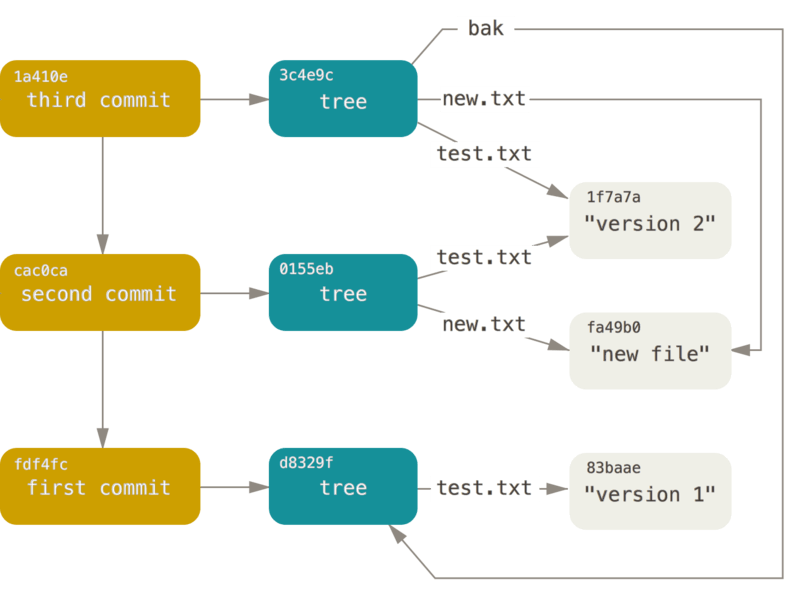
\includegraphics[width=0.8\textwidth]{figs/git-data-model}
  \caption{An example of a possible layout of objects in a Git store containing three commits. Example taken from the Pro Git\cite{chacon2014git}.}
  \label{fig:gitdatamodel}
\end{figure}

\subsection{Porcelain and Plumbing}

Git has two sets of command-line tools: its ``porcelain'' tools and its ``plumbing'' tools. The important difference is that the porcelain tools are the ones that users of the version control system should use for all normal operations but the plumbing tools are lower level and allow direct interaction with the Git store. As I am using the Git store in slightly non-standard ways, it was important to learn the plumbing commands so that I can use the full power of the Git storage system while simultaneously leaving the Git store in a valid state after each operation. A further description of the differences can be found in the Git book\cite{chacon2014git}.

\section{ocaml-git}

One library that my project relies heavily on is ocaml-git\cite{code_ocaml-git}. It is a complete reimplementation of the Git specification in OCaml. This is very useful as it provides immediate interoperability with my code rather than having to write wrappers for shell scripts whenever I wish to interact with a Git store. However, a downside is that it is much lower level in terms of what it offers than the Git command-line interface. It offers types and modules that allow reading, writing and modifying any type of Git object in a Git store. It also offers some interaction with the index. However, it does not add any other features which means that any features of the Git porcelain commands must be reimplemented as required. This is also true for quite a few of the operations that the standard plumbing commands offer. I planned to use it as a means of interacting with Git stores without having to worry about their layout on disk so that I can focus more on functionality.

\section{Maildir}

As I had chosen Maildir as the kind of email storage I was going to model, it was important to find out its exact specification in terms of structure and interaction. Maildirs seem at a first glance to be incredibly simple and this is because they have been built to look that way to any email client to make interoperability easier. However, this works because they exploit tricks of the filesystem. Namely, they are reliant on filesystem operations being atomic otherwise things start to break down when it comes to concurrent reads and writes (it becomes possible for two processes to start writing the same file at the same time due to inability to check name collisions).
Each email is stored as a separate file with a unique name. These emails are then stored in one of three directories:

\begin{itemize}
\item \texttt{tmp}: Emails are stored here while being delivered
\item \texttt{new}: Emails that have been delivered but not read are stored here
\item \texttt{cur}: All other emails are stored here
\end{itemize}

Also, flags can be added to the end of email filenames to provide extra metadata such as if an email has been flagged for follow up. Furthermore, there are specific rules about the structure of the names and how the randomness should be generated for them to provide enough safety from name collisions. There are also rules about how exactly an email should be delivered to the directory to be safer in concurrent situations. The exact specifications can all be found in the original document written by its creator\cite{bernstein2000maildir}.

There are many extensions to the standard providing extra features such as:

\begin{itemize}
\item Notation for email subdirectories (subdirectores are \texttt{.name} and are themselves a Maildir).
\item Mailbox quotas to add size restrictions (part of Maildir++)
\end{itemize}

All of these features had to be taken into account for the implementation, but given the new storage structure, some of the rules proved irrelevant such as the \texttt{tmp} directory for deliveries with relinking to \texttt{new} because all the concurrency issues are instead handled with locking and Git. The exact details of the mapping in the implementation can be found in section \ref{section:mapping}.

\section{Plan Refinement}

The original plan specified that the project would consist of a Git overlay for Maildir where filesystem operations would be bundled into commits. It also specified that some possible extensions would be implemented using Git's branching model and by parsing emails themselves. To further refine this it was necessary to perform a requirements analysis to decide which features the result would need so that then the implementation strategy could be confirmed.

\subsection{Requirements}

Before starting the project, it was necessary to work out exactly which features needed to be implemented for a functioning mailbox. This was done by looking a what operations can take place and any extra features the Maildir standard has. A mailbox is used at two different times, when email is delivered, and when it is accessed. This can be by the same or different applications. This means I must support delivery and the operations that may be performed by an access. When email is accessed, this is so that it can be read by an application, so retrieval must be supported. Also, the Maildir standard allows for flags (ie metadata) to be set on an email. Therefore a way to perform this must also be supported. Finally, there must be a way to see what emails exist so that the above operations can be performed. The operations chosen for implementation based on these points are below:

\begin{itemize}
  \item Email delivery
  \item Email retrieval (for reading)
  \item Email metadata modification (through changing flags)
  \item Email deletion.
\end{itemize}

As my success criteria specified that my project should support all standard Maildir operations, I made all of these operations required features of the final application. I also decided that there were some more features that would be useful to have which are described in the next section.

\subsection{Plan modifications and clarifications}

Given the above requirements, further to the initial plan it was decided that it would be useful for the library to also work on standard Unix-based operating systems such as Linux, BSD and macOS. Therefore it was necessary to also implement a command-line tool to interact with a Gitmaildir. Furthermore, I realised that it would be very useful to have a daemon to synchronise a Gitmaildir with a standard Maildir allowing common email applications to interface with it without them needing to be modified themselves, so this was another feature not in the plan that was to be built in the implementation. Other than these, the plan was otherwise unchanged.

I also decided that alongside the success criteria it would be useful to evaluate the performance of a Gitmaildir against those of an Mbox and Maildir as this is an important metric related to whether it is actually a usable alternative. It is not enough that it works correctly if it is still too slow to compete with these widely-used standards.

\section{Professional practice}

To make sure that the project went smoothly I decided to adopt some best practices. These included unit testing. Alongside writing code for the library, I chose a unit test framework allowing for me to write tests for each component of the library which I could run to check the expected behaviour after each new set of changes. The benefit of this is to be able to see if any changes have unexpected consequences in modifying the behaviour of the application.

So that it would be easier for other people to use the library I decided that I would add documentation for every function. These would be in the form of ocamldoc doc strings. The reason for doing it like this is that the documentation lives with the code and so it is easily accessible to those using and modifying the code. Another benefit is that API documentation in many formats (eg HTML) can be easily generated using a single command when needed.

In addition to documentation it is important that the code itself is readable. So that this was the case I decided to follow the OCaml style guidelines\cite{ocaml_guidelines} meaning that my code would be readable to anyone that is familiar with what common OCaml code looks like. In cases where elements I was using were less standard I decided that I would aim to try to be consistent with any examples from the library originator. When no such samples existed I decided to aim to at least be consistent with myself.

To ensure that I would be safe from catastrophic loss of project code I decided to keep it backed up at all times. The service I chose for this was Github. This was chosen as it is widely used by developers and comes with the further benefit of using Git. This also means that I had access to a history of changes so that it would be easy to roll back changes if they turn out not to be quite right.
